\hspace*{1cm}Энэ бүлэгт судалгааны ажлын онолын үндэслэл, холбогдох бүтээлүүдийн тоймыг танилцуулна. Үүний хүрээнд микрофронтенд архитектурын ойлголт, ISO/IEC 25010 стандарт, мөн сүүлийн үеийн ижил төстэй судалгаануудыг тус тус авч үзэх болно.
\section{Онолын судалгаа}
Энэ хэсэгт судалгааны сэдэв, асуудал, даалгаврыг ойлгоход шаардлагатай үндсэн ойлгол- туудын тодорхойлолт, тайлбарыг танилцуулах болно. Микрофронтенд гэх ойлголтыг таниу- лахын тулд вэб хэрэглээний программ хөгжүүлэлтийн одоогийн хандлагууд, микросервис архитектурын үндсэн зарчмуудыг тайлбарласнаас гадна тестийн үр дүнг үнэлэхэд анхаарч үзсэн ISO/IEC 25010 стандарт, чанарын үзүүлэлтүүдийг мөн дурдсан болно.
\subsection{Цул архитектур}
Төслийн цар хүрээ тэлэхийн хэрээр модулиуд хоорондоо улам их хамааралтай болж эхлэн, нарийн төвөгтэй байдал нэмэгдэж, аль нэг модульд өөрчлөлт оруулах нь бусад модулиудад урьдчилан таамаглах аргагүй үр дагавар авчрах эрсдэлтэй болдог. Энд зөвхөн код цул болоод зогсохгүй, бусад хөгжүүлэгчидтэй хамтран ажиллах эсвэл шинэ хөгжүүлэгч багт нэмэгдэхэд хүндрэлтэй болдог. Зураг \ref{fig:mono}.а-д цул архитектуртай хэрэглээний программын давхаргуудыг харуулав.

\begin{figure}[h!]
	\centering
	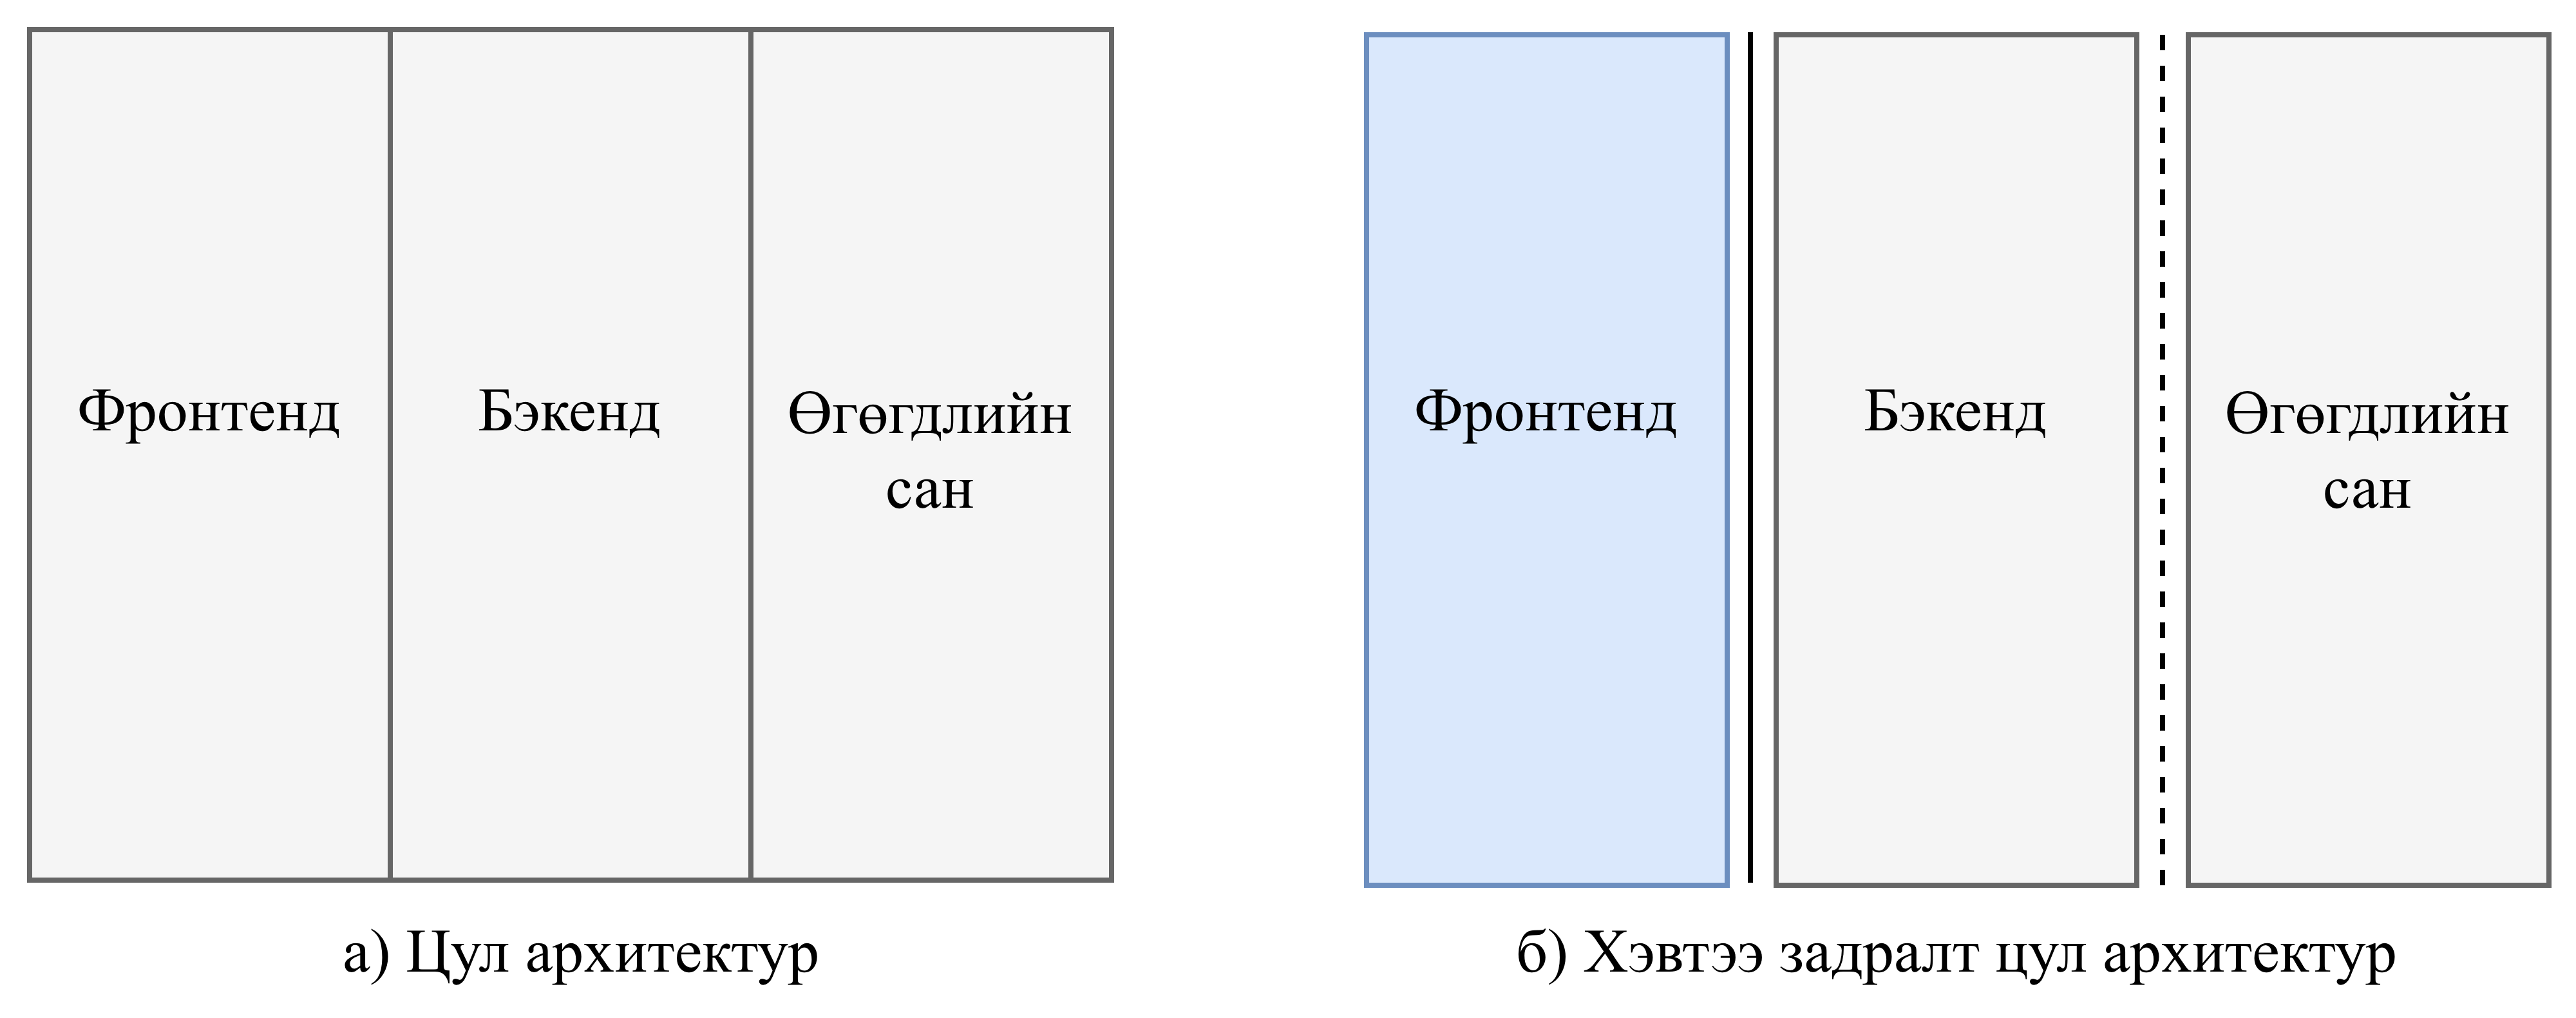
\includegraphics[width=16cm]{images/mono.png}
	\caption{Цул архитектур}
	\label{fig:mono}
\end{figure}

Үүний улмаас хөгжүүлэлтийн процессыг фронтенд, бэкенд, өгөгдлийн сангийн давхарга \cite{geers2017} гэх мэтээр хэвтээ чиглэлд задалдаг. Ингэж задалснаар зөвхөн код өөр өөр давхаргад хуваагдаад зогсохгүй, хөгжүүлэлтийн багууд ч тухайн хөгжүүлэлтийн чиглэл болон ашиглаж буй технологиороо хуваагдах боломжтой болдог. Зураг \ref{fig:mono}.б-д Geers-ийн \cite{geers2017} тайлбарласан хэвтээ задлалтыг харуулсан болно. Өөр өөр давхаргад задалсан хэдий ч хэрэглээний программ томорч, нарийн төвөгтэй болох тусам цул программ хангамжийн хөгжүүлэлт байсаар байдаг. \cite{dragoni2017}-т дурдсанаар цул архитектур нь дараах олон асуудлыг дагуулдаг:
\begin{itemize}
		\item Засвар үйлчилгээ, хөгжүүлэх, алдааг хянахад хүндрэлтэй.
		\item Сан нэмэх, шинэчлэхэд код ажиллахгүй болох, тааварлашгүй байдлаар ажиллах эрсдэлтэй.
		\item Өөрчлөлт оруулахын тулд бүхэл хэрэглээний программыг дахин нэвтрүүлэх шаардлагатай болдог.
		\item Байршуулалтийн тохиргоо нь бүх бүрэлдэхүүн хэсэгт тохирсон байх ёстой.
		\item Өргөтгөх боломж хязгаарлагдмал байдаг.
		\item Сонгосон технологи, фреймворкийг л үргэлжлүүлэн ашиглах шаардлагатай болдог.
\end{itemize}

Нөгөөтэйгүүр Atlassian \cite{atlassian_microservices} цул архитектурын дараах давуу талуудыг онцолсон:
\begin{itemize}
	\item Бүхэл бүтэн хэрэглээний программыг нэг л файл ашиглан нэвтрүүлдэг.
	\item Хэрэглээний программ нэг кодын сан дээр суурилан бүтээгддэг.
	\item Модулиуд хоорондоо нэг процесс дотор ажилладаг тул API дуудлага хийхэд илүү хурдан.
	\item Нэг кодын санд байдаг тул тестлэхэд хялбар бөгөөд E2E тестлэхэд тохиромжтой байдаг.
	\item Хэрэглээний программ илүү энгийн үед хүсэлтүүдийг мөшгөх, асуудлыг олоход хялбар байдаг.
\end{itemize}

\subsection{Микросервис архитектур}
\label{sec:microservices}
Микросервис архитектур нь бие даан нэвтрүүлэх боломжтой үйлчилгээнүүд дээр тулгуур- ладаг архитектур юм \cite{atlassian_microservices}. Эдгээр үйлчилгээ бүр нь өгөгдлийн сантай байж болно \cite{dragoni2017}. Үйлчил- гээнүүд хоорондоо хөнгөн протоколууд ашиглан харилцдаг \cite{blinowski2022}. Микросервисийг ойлгохын тулд энэхүү архитектурыг бүрдүүлдэг дараах хэд хэдэн үндсэн зарчмуудыг мэдэх хэрэгтэй:
\begin{enumerate}
	\item Сул холбоост буюу бусад микросервисүүдэд нөлөөлөхгүйгээр аль нэг микросервист өөрчлөлт оруулах боломжтой байх.
	\item SOLID\cite{blinowski2022} зарчмын дагуу үйлчилгээ бүр зөвхөн нэг л үүрэг хариуцлагатай байх ёстой.
	\item Үйлчилгээнүүд нь бие даасан бөгөөд бүх хамаарлуудыг өөртөө агуулсан байдаг.
	\item Үйлчилгээний төгсгөлийн цэгүүд нь API хэлбэрээр ил гарсан байдаг. API нь хийсвэрлэл үүсгэдэг бөгөөд бусад үйлчилgээнүүд нь тухайн үйлчилgээнд ашиглагдаж буй технологи, бүтэц, логик хэрэгжүүлэлтийн талаар мэдэх шаардлагагүй байдаг.
\end{enumerate}

Kubernetes \cite{dragoni2017}, Docker \cite{ponce2019} гэх мэт хэрэгслүүд нь бэкенд хөгжүүлэгчдэд микросервисүүдийг ашиглах, удирдан зохион байгуулахад тусалдаг. Geers \cite{geers2017} хөгжүүлэлтийн өнөөгийн чиг хандлага бол микросервис бэкенд дээр суурилсан SPA (Single Page Application) фронтенд гэж тайлбарласан байдаг (Зураг \ref{fig:micro}).
\begin{figure}[h!]
	\centering
	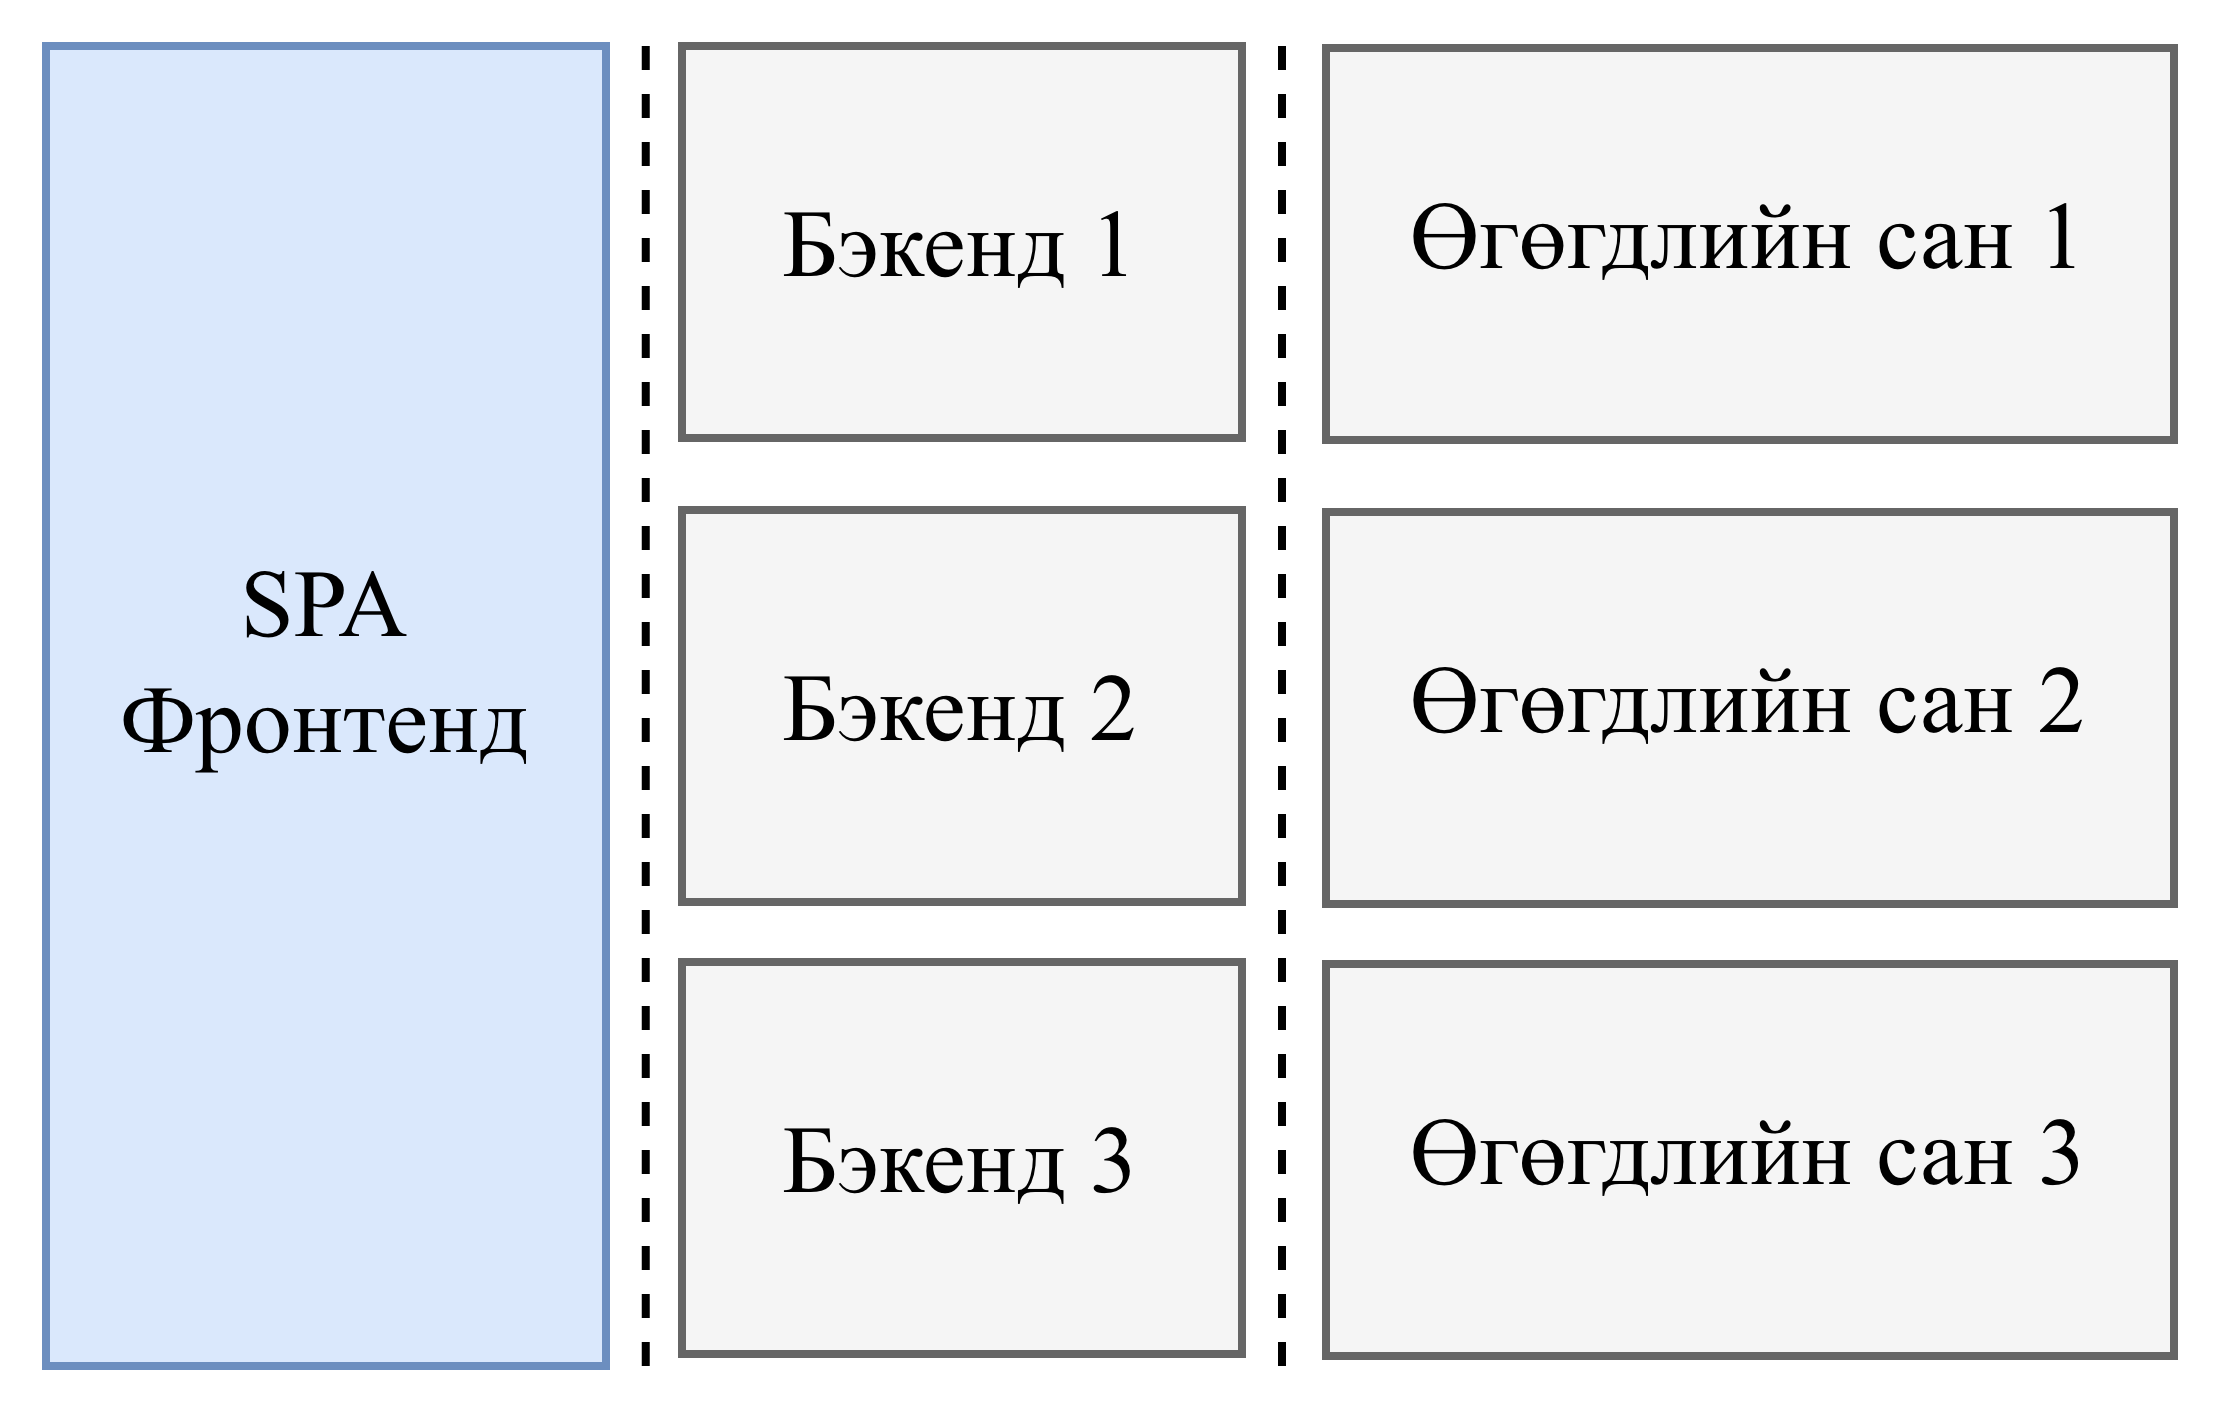
\includegraphics[width=8cm]{images/micro.png}
	\caption{Микросервис архитектур}
	\label{fig:micro}
\end{figure}
\cite{atlassian_microservices}-р нийтлэлд Atlassian компани дараах давуу талуудыг онцолжээ:
\begin{itemize}
	\item Жижиг багуудаар Шалмаг аргачлалаар ажиллах.
	\item Үйлчилгээний инстанц үүсгэх нь маш хурдан байдаг.
	\item Инстанц бүрийг бие даан нэвтрүүлдэг тул бусад бүрэлдэхүүн хэсгүүдийг дахин нэвтрүү- лэх шаардлагагүй. Энэ нь хөгжүүлэлтийн амьдралын мөчлөгийг хурдасгадаг.
	\item Алдааг тусгаарлаж, засахад хялбар байдаг. Кодын шинэчлэлт хийх, шинэ боломжууд нэвтрүүлэх нь хамаагүй хурдан болдог.
	\item Шинэ фичер бүхий бие даасан нэгжүүдийг хялбархан нэвтрүүлж болно.
	\item Багууд өөрсдийн хүссэн хэрэгсэл, технологийг сонгох боломжтой.
	\item Өөрчлөлтийг нэвтрүүлэх нь бүхэл бүтэн хэрэглээний программыг унагах эрсдэл үүсгэдэггүй.
	\item Багууд илүү бие даасан болдог.
\end{itemize}

Нөгөө талаас, Харрис өөрийн нийтлэлдээ [9] микросервис архитектурын сул талыг дурджээ:
\begin {itemize}
	\item Олон тооны микросервисүүдийг удирдах нь бэрхшээлтэй бөгөөд үүнийг зөв хийхгүй бол хөгжүүлэлтийг удаашруулах эрсдэлтэй.
	\item Микросервис бүр тест, байршуулалт, хостинг, хяналт зэрэг өөрийн гэсэн зардалтай байдаг.
	\item Шинэчлэлтүүдийг зохицуулахын тулд багууд харилцаа холбоо, хамтын ажиллагааны шинэ түвшнийг нэмэх шаардлагатай болдог.
	\item Нэг бизнесийн логик нь хэд хэдэн инстанц дундуур дамжин ажиллах боломжтой бөгөөд энэ нь алдааг олж засахад хүндрэл учруулдаг.
	\item Микросервис бүрд зориулсан нийтлэг платформ байдаггүй тул лог хөтлөх стандарт, хяналт зэргийг ижил түвшинд хэрэгжүүлэхэд хэцүү байдаг.
	\item Нэг баг олон микросервис эзэмшиж болдог тул тухайн микросервисийг аль баг хариуцдаг нь тодорхойгүй байх үед дэмжлэг үзүүлэхтэй холбоотой асуудлуудыг үүсгэдэг.
\end{itemize}

\subsection{Нэг хуудаст хэрэглээний программ (SPA)}
\hspace*{1cm}Миковски болон Пауэлл нар өөрсдийн номондоо \cite{mikowski2013} SPA-г вэб хэрэглээний программ хөгжүүлэл- тийн шинэ, орчин үеийн архитектурын арга барил хэмээн тодорхойлсон байдаг. SPA нь агуулгаа динамикаар шинэчилдэг вэб хэрэглээний программ юм. Энэ нь өөрчлөгдсөн харагдацын хэс- гүүдийг л шинэчилж, харуулдаг. SPA нь серверээс өгөгдөл татахын тулд AJAX хүсэлтүүдийг ашигладаг. SPA архитектур нь Angular, Vue, React гэх мэт хамгийн алдартай фреймворкуудад хэрэгжсэн байдаг. SPA архитектурын сул тал нь кодын сан томрох тусам түүнийг арчлах, шинэ боломжууд нэмэхэд илүү хэцүү болдог. Энэ нь ихэвчлэн бүхэл бүтэн хэрэглээний программыг дахин бичих эсвэл дахин зохион байгуулахад хүргэдэг.
\subsection{Микрофронтенд архитектур}
Микросервис архитектурыг фронтенд хөгжүүлэлтэд нэвтрүүлэх нь байршуулалт, хөгжүү- лэлт, багийн зохион байгуулалт зэрэгт шинэ боломжуудыг олгодог. Микрофронтенд архитек- турыг бий болгохын тулд тэдгээр Микросервис архитектурын зарчмуудыг (Дэд бүлэг \ref{sec:microservices}-ыг үзнэ үү) хэрэгжүүлэх нь чухал юм. Зураг \ref{fig:microfrontend}-т  микрофронтенд хөгжүүлэлтийн хандлагыг харуулав. Энэ хандлага нь фронтендийг удирдах боломжтой бүрэл- дэхүүн хэсгүүдэд задлах бөгөөд бүрэлдэхүүн хэсэг бүр нь тодорхой бизнесийн логикийг хариуцдаг. Фронтенд бүрэл- дэхүүн хэсэг бүр API ашиглан бэкендтэй харилцдаг бөгөөд энэ нь өөр өөрийн фронтенд кодын сантай байдаг. Микрофронтенд архитектурт \textit{хэвтээ} задлалтаас зайлсхийх хэрэгтэй \cite{fowler_microfrontends}. Энд багуудыг микрофронтенд хэрэглээний программуудаар нь хуваах хэрэгтэйг онцолсон байдаг. Багууд нь \textit{босоо} чиглэлд бүрэлдэх ёстой бөгөөд баг бүр нэг микро хэрэглээний программыг хариуцаж, тодорхой нэг фичерийг хөгжүүлж нийлүүлэх үүрэгтэй байдаг.

\begin{figure}[h!]
	\centering
	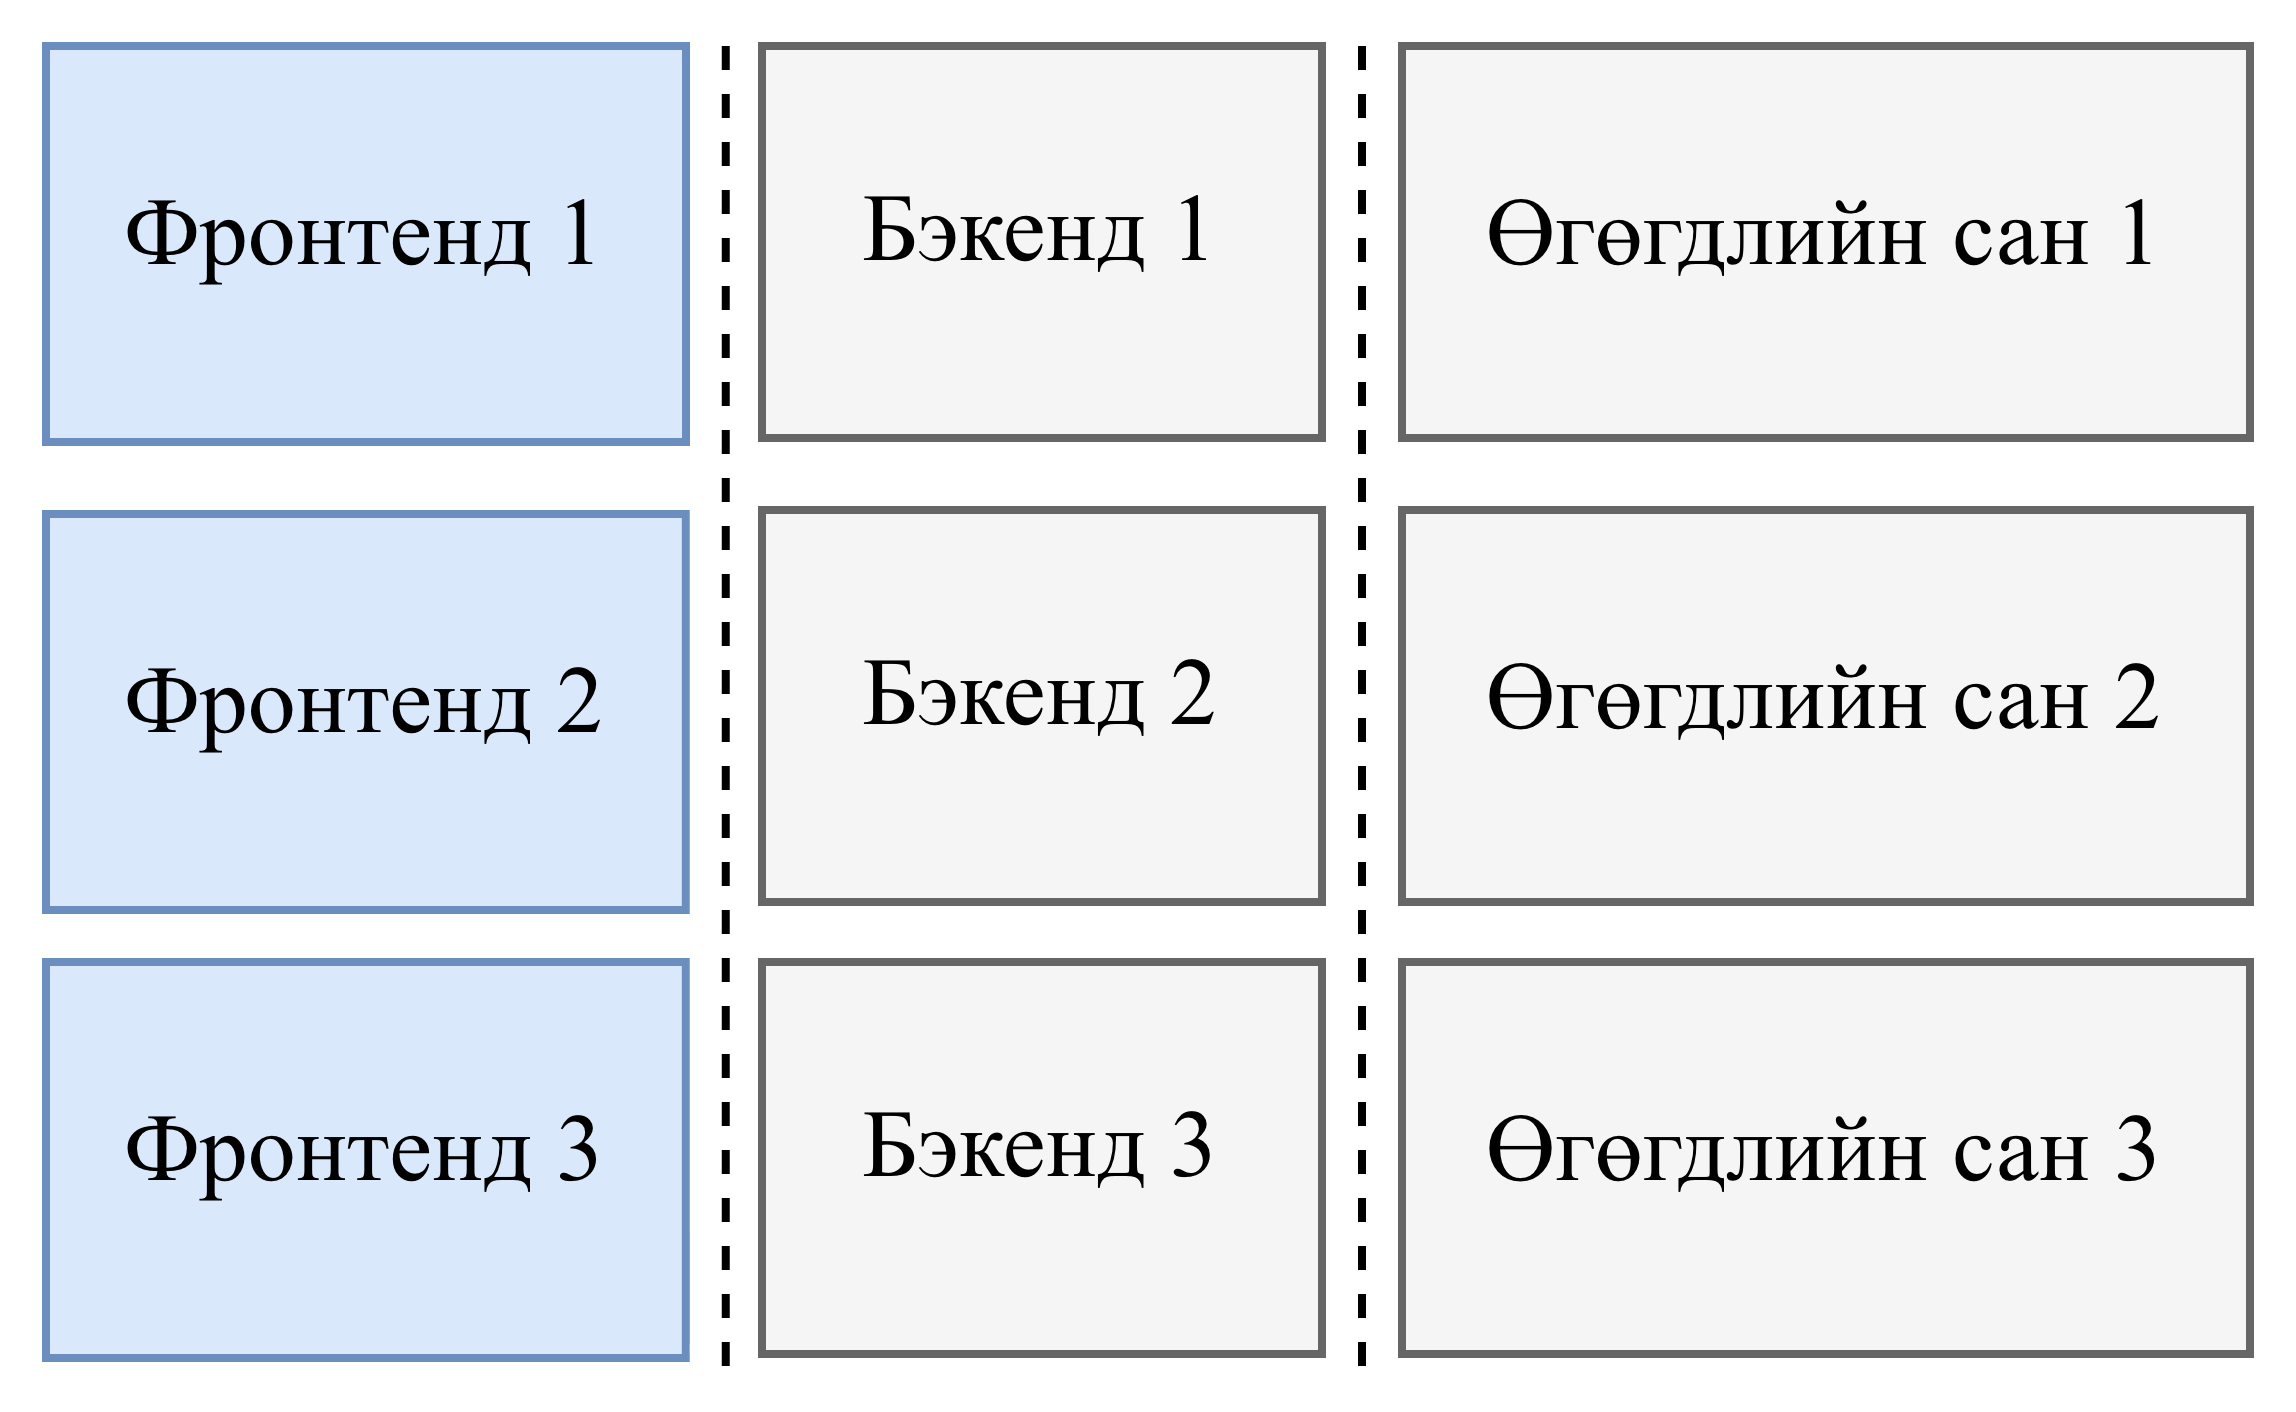
\includegraphics[width=8cm]{images/microfrontend.png}
	\caption{Микрофронтенд архитектур}
	\label{fig:microfrontend}
\end{figure}

Мартин Фаулер \cite{fowler_microfrontends} микрофронтенд архитектурыг ашиглахын давуу талуудыг дурджээ:
\begin{itemize}
	\item Хэрэглэгчдэд шинэ боломжуудыг үргэлжлүүлэн хүргэхийн тулд хуучин кодын санг хөгжүүлэх явцдаа хэсэг хэсгээр нь шинэчлэн бичих боломжтой.
	\item Жижиг кодын сангууд дээр ажиллахад илүү хялбар байдаг. Санамсаргүй хамаарал (coupling) үүсгэхгүйн тулд бүрэлдэхүүн хэсгүүдийн хоорондох хил хязгаарыг тодорхой болгодог.
	\item Кодын сан бүр өөрийн гэсэн нийлүүлэлтийн дамжлагатай бөгөөд энэ нь кодыг бүтээх, тестлэх, продакшн руу нэвтрүүлэх ажлыг хийдэг. Нэг бүрэлдэхүүн хэсгийг унагах боломжтой тул алдаа гарах үед учрах эрсдэл бага байдаг.
	\item Багууд нь бие даасан бөгөөд бүх давхаргаа (фронтенд, бэкенд, өгөгдлийн сан) бүрэн хариуцдаг. Энэ нь хөгжүүлэлт болон шинэ боломжуудыг нэвтрүүлэх процессыг илүү хялбар, хурдан болгодог.
\end{itemize}

Товчхондоо микрофронтенд гэдэг нь том кодын санг жижиг, удирдаж болохуйц хэсгүүдэд хувааж, тэдгээрийн хоорондын хамаарлыг тодорхой болгохыг хэлнэ. Харин сул талуудыг дараах байдлаар онцолжээ:
\begin{itemize}
	\item Давхардсан сангууд нь өөр өөр микрофронтенд хэрэглээний программуудад ачаалагддаг тул илүү их нөөц зарцуулах эрсдэлтэй.
	\item Локал хөгжүүлэлт болон продакшн орчны хоорондох ялгаатай байдал.
	\item Олон микрофронтенд хэрэглээний программтай болох нь удирдах, арчлах олон домэйн, сервер, хэрэгслүүдтэй болоход хүргэдэг.
\end{itemize}

\subsection{Интеграцийн төрлүүд}
\label{sec:integration-types}
Мартин Фаулерын \cite{microfrontends_info} нийтлэлд интеграци хийх хугацааны хувьд хоёр төрлийн интегра- цийг ялгаж үздэг. Интеграцийн хугацаа гэдэг нь микрофронтенд ашиглаж буй хэрэглээний программ тухайн микрофронтендийн эх код руу нэвтрэх эрхтэй болох цаг мөчийг хэлнэ. Микрофронт- ендийг дээрх хоёр төрлийн цаг хугацааны интеграцийн аль алинд нь хэрэгжүүлэх боломжтой. Гэхдээ тэдгээр нь бүгд микросервисийн үндсэн зарчмуудыг хангадаггүй.
\subsubsection{Угсралтын үеийн интеграци (Build-time integration)}
\hspace*{1cm}Угсралтын үеийн интеграци нь заримдаа компиляци интеграци (compile-time) гэж бас нэр- лэгддэг бөгөөд энэ нь микрофронтендийг импортолж буй хэрэглээний программ хөтөч дээр ачаалаг- дахаас өмнө ашиглагдах микрофронтендийн эх код нь нэгтгэгдсэн байхыг хэлнэ. Энэхүү интеграцийг микрофронтендийг npm багц хэлбэрээр нийтэлж, дараа нь үндсэн хэрэглээний программ рүү хамаарал болгон импортлох замаар хэрэгжүүлэх боломжтой. Микрофронтенд архитек- турыг нэвтрүүлэхэд энэ хандлагыг ашиглах нь ойлгоход илүү хялбар боловч микрофронтенд архитектурын үндсэн бүх зарчмыг хангаж чаддаггүй. Аль нэг npm багцад өөрчлөлт орох бүрд тэдгээр багцыг импортолсон микрофронтенд хэрэглээний программуудыг мөн дахин нэвтрүүлэх шаардлагатай болдог. Энэ үед микрофронтендүүд сул холбоост байж чадахгүй бөгөөд импор- толсон микрофронтендүүдээсээ илүү их хамааралтай, нягт холбоотой болдог.
\subsubsection{Ажиллах үеийн интеграци (Run-time integration)}
\hspace*{1cm}Ажиллах үеийн интеграцийг сервер талын (server-side), клиент талын (client-side) болон захын (edge-side) интеграци гэж гурван дэд ангилалд хуваадаг \cite{microfrontends_info}. Ажиллах үеийн интеграци гэдэг нь микрофронтендийг импортолж буй хэрэглээний программ хөтөч дээр ачаалагдсаны дараа ашиг- лагдах микрофронтендийн эх код нэгтгэгдэхийг хэлнэ. Энэ төрлийн интеграцийг тохируулахад илүү төвөгтэй байдаг. Микрофронтендүүдийн хувьд илүү их тохиргоо шаарддаг. Нөгөө талаас, хэрэгжүүлэлтийн энэ арга нь микрофронтендүүдийн сул холбоост байдлыг бий болгодог. Микрофронтендүүдийн байршуулалтыг бие даан хийх боломжтой бөгөөд бүхэл бүтэн аппли- кэйшнийг дахин нэвтрүүлэх шаардлагагүй болдог. Захын болон сервер талын интеграци нь илүү их нөөц шаарддаг тул энэхүү ажилд бэлтгэсэн демо загвар болон шилжүүлэлтэд клиент талын интеграцийг ашиглах болно.

Тодорхойлсон интеграцийн төрлүүд дээр үндэслэн микрофронтенд архитектурын аль үндсэн зарчмуудыг хангаж байгааг Хүснэгт \ref{tab:integration_types}-д харуулав. 
\begin{table}[H]
\centering
\caption{Интеграцийн төрлүүдийн харьцуулалт}
\label{tab:integration_types}
\renewcommand{\arraystretch}{0.7}
\begin{tabular}{lcc}
\toprule
\textbf{Үндсэн зарчмууд} & \textbf{Build-time} & \textbf{Run-time} \\
\midrule
Нэг хариуцлагатай (Single responsibility) & x & x \\
Бие даан нэвтрүүлэх боломжтой (Independently deployable) & & x \\
Фреймворкоос үл хамаарах (Framework agnostic) & x & x \\
Сул холбоост (Loosely coupled) & & x \\
\bottomrule
\end{tabular}
\end{table}

\section{Сэдвийн судалгаа}
\label{sec:literature-review}
Энэ хэсэгт микрофронтенд архитектур зохиомж, түүний янз бүрийн шинж чанар, хэрэгжүү- лэлт болон өмнө нь хийгдсэн судалгааны ажлуудын тоймыг хүргэх болно. Одоо байгаа ном зохиол, судалгааг тоймлохын гол зорилго нь микрофронтенд архитектур зохиомжтой холбоотой орчин үеийн тэргүүлэх шийдлүүд,  холбогдох хэрэгсэл, багц, санг судлахад оршино.
\subsection{Судалгааны ажлын хайлт}
\hspace*{1cm}Холбогдох өгүүллүүдийг олохын тулд Scopus\footnote{Scopus нь шинжлэх ухааны сэтгүүл, ном, хурлын бүтээлийн хураангуй болон эшлэлийн мэдээллийг нэгтгэсэн олон улсын хамгийн том өгөгдлийн сан юм.}, DiVA\footnote{DiVA нь магистр болон докторын зэрэг хамгаалах ажил, судалгааны бүтээл, нийтлэл, сэтгүүл зэрэг шинжлэх ухааны бүтээлүүдийн цуглуулга бүхий сан юм.} өгөгдлийн санг ашигласан. Хайлтын утгад микрофронтенд архитектур зохиомжийн нэршлийн өөр өөр хувилбаруудыг ашигласан болно. Үүнд: \verb|micro-фронтенд| \verb|OR| \verb|microfrontend| \verb|OR| \verb|"micro фронтенд*"**| гэсэн хайлтын утгаар Scopus өгөгдлийн сангаас нийт 47 илэрц, \verb|microfrontend| \verb|OR| \verb|micro фронтенд| \verb|OR| \verb|micro-фронтенд| гэсэн хайлтын утгаар DiVA сангаас 5 илэрц олдсон. Өгүүллийн гарчиг, хураангуй, эсвэл түлхүүр үгсэд хайлтын утга орсон бүтээлүүдийг сонгож авсан. Олдсон өгүүллүүдийг уншиж танилцсаны дараа судалгааны арга зүй, сэдвийн хамаарал, сэдвийг хэрхэн хөндсөн байдал зэрэгт нь үндэслэн 5 өгүүллийг тоймлон үзэхээр сонгосон. Эдгээрийн 1 нь DiVA сангаас, үлдсэн 9 нь Scopus өгөгдлийн сангаас авагдсан болно.

\subsection{Сонгож авсан судалгааны ажил}
\hspace*{1cm}\cite{mohammed2022} дугаартай бүтээлд зохиогчид нь одоо ашиглагдаж буй QL4POMR бэкенд программ хангамжийн шийдэл дээр тулгуурлан эмч, өвчтөн хоорондын харилцан яриаг загварчлах зориулалттай чатботыг хэрхэн хэрэгжүүлсэн талаар тайлбарласан байдаг. Энэхүү харилцан ярианы систем нь patientMFE болон physicianMFE гэж нэрлэгдсэн хоёр микрофронтенд аппли- кэйшнээс бүрдэнэ. Уг бүтээлд микрофронтенд хэрэгжүүлэхэд ашиглагддаг Piral, SystemJS, Single SPA, Webpack Module Federation, Bit.Dev зэрэг зарим хэрэгслүүдийг дурджээ. Хэрэг- жүүлэлтийн техникийн шийдэл нь зөвхөн тухайн системийн тохиргоонд зориулан ашигласан технологиудаар хязгаарлагдсан байна.
\newline
\hspace*{1cm}\cite{stefanovska2022} дугаартай бүтээлд Стефановска болон Трайковик нар домэйнд суурилсан зохиомж нь микрофронтенд архитектурын үндсэн гол ойлголт болохын хувьд түүний тоймоор судал- гаагаа эхлүүлсэн байна. Тэд одоо байгаа техникийн шийдлүүдийг чанарын үзүүлэлтүүд ашиглан үнэлжээ. Үнэлгээ хийсний дараа тэд кодын дахин ашиглалтыг чухалчилсан өөрсдийн техникийн шийдлээ санал болгосон. Энэхүү техникийн шийдэл нь 2 ажлын явцаас бүрдсэн. Эхний ажлын явцад вэб компонент нь фронтенд хэрэглээний программыг бүхэлд нь агуулах бүрхүүл байдлаар хэрхэн ажилладгийг тайлбарласан. Хоёр дахь ажлын явц нь модулийн шинж чанарт төвлөрсөн бөгөөд үүнийг Module Federation Plugin ашиглан хэрэгжүүлсэн байна. Тэдний дурдсан Module Federation Plugin-ийг ашигласнаар олж авах боломжтой нэг шинж чанар нь өргөжүүлэх боломж юм. Учир нь микрофронтенд хэрэглээний программуудыг статик JavaScript файл хэлбэрээр татаж авдаг байна. Санал болгосон хэрэгжүүлэлтийн үр дүнд хэрэглээний программын хөгжүүлэлтээс үйлдвэрлэл рүү шилжих амьдралын мөчлөгийн хугацаа илүү хурдан болсон байна.
\newline
\hspace*{1cm}\cite{pavlenko2020} дугаартай бүтээлд вэб хөгжүүлэлт дэх микрофронтенд архитектурын ойлголтуудыг нарийвчлан судалсан байдаг. Зохиогчид үүнийг микросервис архитектурын дараагийн салш- гүй, зүй ёсны хөгжил гэж үзсэн. Уг судалгаанд вэб болон бэкенд хөгжүүлэлтийн уламжлалт болон микросервис архитектурын хандлагуудыг харьцуулж, микрофронтендийн өнөөгийн туршлагуудыг судалжээ. Хөгжүүлэгчдийн туршлагад үндэслэн кэйс судалгаа хийсэн бөгөөд чиглүүлэлт, статик файл дамжуулалт, репозиторын зохион байгуулалт зэрэгт тулгардаг сорил- туудыг онцолсон байна. Микрофронтенд нь том баг, нарийн төвөгтэй, томоохон хэмжээний төслүүдэд илүү тохиромжтой гэж дүгнэсэн. Харин цөөн хөгжүүлэгчтэй багийн хувьд уг архитектурыг дэмжиж ажиллахад нэмэлт хүчин чармайлт шаарддаг бөгөөд төслийн бүтэц, хөгжүүлэлтийн процессыг нэлээд төвөгтэй болгодог байна. Мөн уг архитектурын давуу талыг бүрэн ашиглахын тулд хөгжүүлэгчдээс тодорхой хэмжээний туршлага шаарддаг төдий- гүй нийгэмлэгийн зүгээс үүнийг бүрэн дэмжих "бэлэн шийдлүүд" хомс байгааг дурджээ.
\newline
\hspace*{1cm}\cite{tilak2020} дугаартай өгүүллийн зорилго нь хөгжүүлэлтийн багийн бүтээмжийг нэмэгдүүлэх, нөөцийн зарцуулалтыг сайжруулахад чиглэсэн платформын шийдлийг танилцуулахад оршино. Уг платформ нь нүсэр, нийлмэл программ хангамжийн хөгжүүлэлтийг төвлөрсөн бус арга зүйгээр хөнгөвчлөх бөгөөд микросервис болон микрофронтендийг үүсгэх, ашиглах процессыг дэмждэг. Энэхүү судалгаа нь микросервис болон микрофронтенд архитектурын давуу тал болон сорилтуудыг ерөнхийд нь тоймлон харуулсан. Зэрэгцээ хөгжүүлэлт болон өргөтгөх боломж нь эдгээр архитектурын хамгийн том давуу тал бөгөөд ингэснээр нөөцийг илүү үр дүнтэй ашиглах боломж бүрддэг байна. Мөн фронтендийн хэсгүүдийг алхам алхмаар шинэч- лэх боломж нь уламжлалт цул архитектуртай харьцуулахад хөгжүүлэгчийн бүтээмжийг эрс нэмэгдүүлдэг. Эцэст нь, зохиогчид бүтээгч, хэрэглэгч болон администраторуудад зориулсан гурван хэсэгтэй платформыг санал болгосон нь системийг хөгжүүлэхэд тулгардаг хүндрэл- үүдийг илүү сайн ойлгох, цаашлаад платформын үйл ажиллагааг сайжруулахад чухал түлхэц болжээ.
\newline
\hspace*{1cm}\cite{montelius2021} дугаартай бүтээлд микрофронтендийн талаарх хайгуулын судалгаа хийж, хөгжүүлэгч- дээс ярилцлага авсан байна. Энэхүү судалгаа нь системийн өөрчлөгдөх боломж болон ерөнхий- лөн ашиглагдах байдал зэрэг чанарын үзүүлэлтүүд дээр төвлөрч, микрофронтендийн давуу тал, тулгарч буй асуудлуудыг тодруулахыг зорьжээ. Судалгааны хүрээнд нэг нь SPA, нөгөө нь микрофронтенд архитектур ашигласан хоёр өөр фронтенд хэрэглээний программ хөгжүүлж туршсан байна. Үүний дараа уламжлалт болон микрофронтенд архитектурын аль алинд нь туршлагатай хөгжүүлэгчдээс ярилцлага авч, өөрчлөгдөх боломжийг үнэлэхийн тулд хэд хэдэн хэмжүүр ашиглажээ. Эдгээр өгөгдөлд үндэслэн микрофронтенд архитектурыг сонгох үед анхаарах ёстой эрсдэлүүдийг хэлэлцсэн байна. Эцсийн дүгнэлтдээ Монтелиус ярилцлагын үр дүнг туйлын үнэн гэхээсээ илүүтэйгээр өөр өнцгөөс харсан хандлага гэж үзэх нь зүйтэйг онцолсон бөгөөд туршилтын загваруудаас гарсан үр дүнг бүх SPA болон микрофронтендүүдэд шууд хамаа- руулан ерөнхийлөн дүгнэх боломжгүйг сануулжээ.

\hspace*{1cm}\cite{ameer2024} дугаартай бүтээлд Амеер болон түүний нөхөд SPA болон микрофронтенд архитектурын гүйцэтгэлийн үзүүлэлтүүдийг бодит туршилтаар харьцуулан судалсан байна. Тэд LCP болон TTI зэрэг вэб гүйцэтгэлийн хэмжүүрүүдийг ашиглан микрофронтенд нь багийн бие даасан байдлыг хангадаг боловч сүлжээний ачаалал нь уламжлалт SPA-ээс муу байх эрсдэлтэйг нотолжээ. Энэхүү судалгаа нь микрофронтенд архитектурыг сонгохдоо гүйцэтгэлийн золиосыг зайлшгүй тооцоолох шаардлагатайг сануулснаараа онцлог юм.
\newline
\hspace*{1cm}\cite{silva2024} дугаартай өгүүлэлд Силва нар микрофронтенд архитектурын чиглэлээр хэвлэгдсэн 100 гаруй эрдэм шинжилгээний бүтээлд системчилсэн тойм хийжээ. Уг судалгаагаар микрофронтендийн хамгийн гол давуу тал нь системийг тусдаа байршуулах чадамж болохыг тодорхойлсон байна. Харин цаашид шийдвэрлэвэл зохих гол сорилтуудад хэрэглээний программ хооронд төлөв хуваалцах, аюулгүй байдал болон хэрэглэгчийн баталгаажуулалт зэрэг асуудлууд багтаж байгааг тэд онцлон тэмдэглэжээ.
\newline
\hspace*{1cm}\cite{bjelotomic2024} дугаартай бүтээлд Бжелотомич нар микрофронтенд боловсруулалтын орчин үеийн хэрэгслүүд болох Webpack болон Vite-ийн гүйцэтгэлийг харьцуулан шинжилсэн байна. Тэд хөгжүүлэгчийн бүтээмж болон дотоод орчны билд хийх хурдыг хэмжсэн бөгөөд React орчинд Vite ашиглах нь хөгжүүлэлтийн процессыг эрс хурдасгадаг болохыг харуулсан. Гэсэн хэдий ч энэ нь зөвхөн хөгжүүлэлтийн орчинд хэмжигдсэн бөгөөд үйлдвэрлэлийн ачааллыг бүрэн тооцоолоогүй гэсэн хязгаарлалттай байв.
\newline
\hspace*{1cm}\cite{mannisto2023} дугаартай судалгаанд хуучин уламжлалт цул хэрэглэгчийн интерфейсийг задалж, микрофронтенд архитектур руу шилжүүлэх практик туршлагыг тайлбарласан байдаг. Маннисто нар системийг үе шаттайгаар салгах нь кодын модульчлалыг хэрхэн сайжруулж байгааг үнэлжээ. Уг бүтээл нь хуучин технологиос орчин үеийн архитектур руу шилжих үед тулгардаг саад бэрхшээлүүдийг бодит төсөл дээр харуулснаараа практик ач холбогдолтой юм.
\newline
\hspace*{1cm}\cite{taibi2022} дугаартай өгүүлэлд Тайби болон Меззалира нар микрофронтенд архитектурыг программхангамжийн архитектурын нарийвчилсан өнцгөөс судалсан байна. Тэд микрофронтендүүдийн хоорондын чиглүүлэлт болон өгөгдөл дамжуулах үед үүсэх сүлжээний ачаалал нь системийн нийт гүйцэтгэлд хэрхэн нөлөөлдгийг шинжилжээ. Мөн системийг хэт олон жижиг хэсгүүдэд хуваах нь засвар үйлчилгээний зардлыг нэмэгдүүлж, бүтцийг нийлмэл болгодог болохыг анхааруулсан байна.

\subsection{Сонгож авсан судалгааны ажлын тойм}
Сонгож авсан 10 судалгааны ажлын хөндсөн үндсэн сэдвүүдийг Хүснэгт \ref{tab:related_work_summary}-д нэгтгэн харуулав.

\begin{table}[H]
\centering
\caption{Сонгож авсан судалгааны ажлын тойм}
\label{tab:related_work_summary}
\renewcommand{\arraystretch}{0.7}
\begin{tabular}{lcc}
\toprule
\textbf{Судалгааны чиглэл} & \textbf{Түлхүүр үгс} & \textbf{Эх сурвалж} \\
\midrule

Модульчлал & Monolith to MFE, Reusability, Migration & \cite{mannisto2023}, \cite{pavlenko2020} \\ 
Гүйцэтгэл & ISO 25010, LCP, TTI, Network overhead & \cite{ameer2024}, \cite{taibi2022}, \cite{stefanovska2022} \\ 
Аюулгүй байдал & State management, Auth, Session sharing & \cite{silva2024}, \cite{mohammed2022} \\
Хөгжүүлэгчийн бүтээмж & DX, Parallel development, Build time & \cite{bjelotomic2024}, \cite{tilak2020}, \cite{montelius2021} \\ 
\bottomrule
\end{tabular}
\end{table}

Судалгааны ажлуудыг шинжлэн үзэхэд хэд хэдэн нийтлэг ололт болон хязгаарлагдмал байдлууд ажиглагдаж байна. Тухайлбал, \cite{mannisto2023}, \cite{pavlenko2020} зэрэг бүтээлүүдэд уламжлалт цул системийг задлах онолын арга зүйг судалсан ч хуучин төлөв хадгалдаг системийг орчин үеийн микрофронтендтэй уялдуулах бодит техникийн шийдэл дутмаг байна. \cite{ameer2024}, \cite{taibi2022}, \cite{stefanovska2022} зэрэг судалгаанууд нь микрофронтендийн сүлжээний саатлыг амжилттай хэмжсэн ч холимог орчин дахь серверийн нөөцийн давхардлыг тооцоолоогүй орхигдуулжээ. \cite{silva2024}, \cite{mohammed2022} зэрэг судалгаанууд микрофронтенд хооронд төлөв хуваалцахыг гол сорилт гэж онцолсон ч төлөв хадгалдаг болон төлөвгүй архитектур хоорондын интеграцийн бодит шийдлийг санал болгоогүй. \cite{bjelotomic2024}, \cite{tilak2020}, \cite{montelius2021} зэрэг судалгаанууд нь зэрэгцээ хөгжүүлэлтийн хурдыг хэмжсэн ч хоёр өөр технологийг нэгэн зэрэг удирдах үед хөгжүүлэгчид үүсэх танин мэдэхүйн ачааллыг үнэлээгүй орхисон байна.

\section{ISO 25010 стандарт}
\label{sec:iso25010}
Программ хангамж болон компьютерын системүүдэд хамаарах бүтээгдэхүүний чанарын үзүүлэлтүүдийг ISO/IEC 25010 стандартад заасан байдаг. Чанарын үзүүлэлтүүд (Quality attri- butes буюу QA) нь олон төрлийн программ хангамжийн шийдэл, хэрэглээний программыг тодорхойлох, хэмжих болон үнэлэхэд ашиглагддаг давтагдашгүй, нарийн тодорхой нэр томьёонууд юм. Энэхүү судалгааны тухайд, тестийн үр дүнг хэмжихийн тулд тус стандартаас хэсэг бүлэг чанарын үзүүлэлтүү- дийг сонгож авсан. Зураг \ref{fig:qa}-т бүтээгдэхүүний чанарын загварыг нийт үзүүлэлт, тэдгээрийн ангиллын хамтаар харуулахын сацуу тусгайлан сонгосон үзүүлэлтүүдийг мөн багтаан харууллаа.
\begin{figure}[h!]
	\centering
	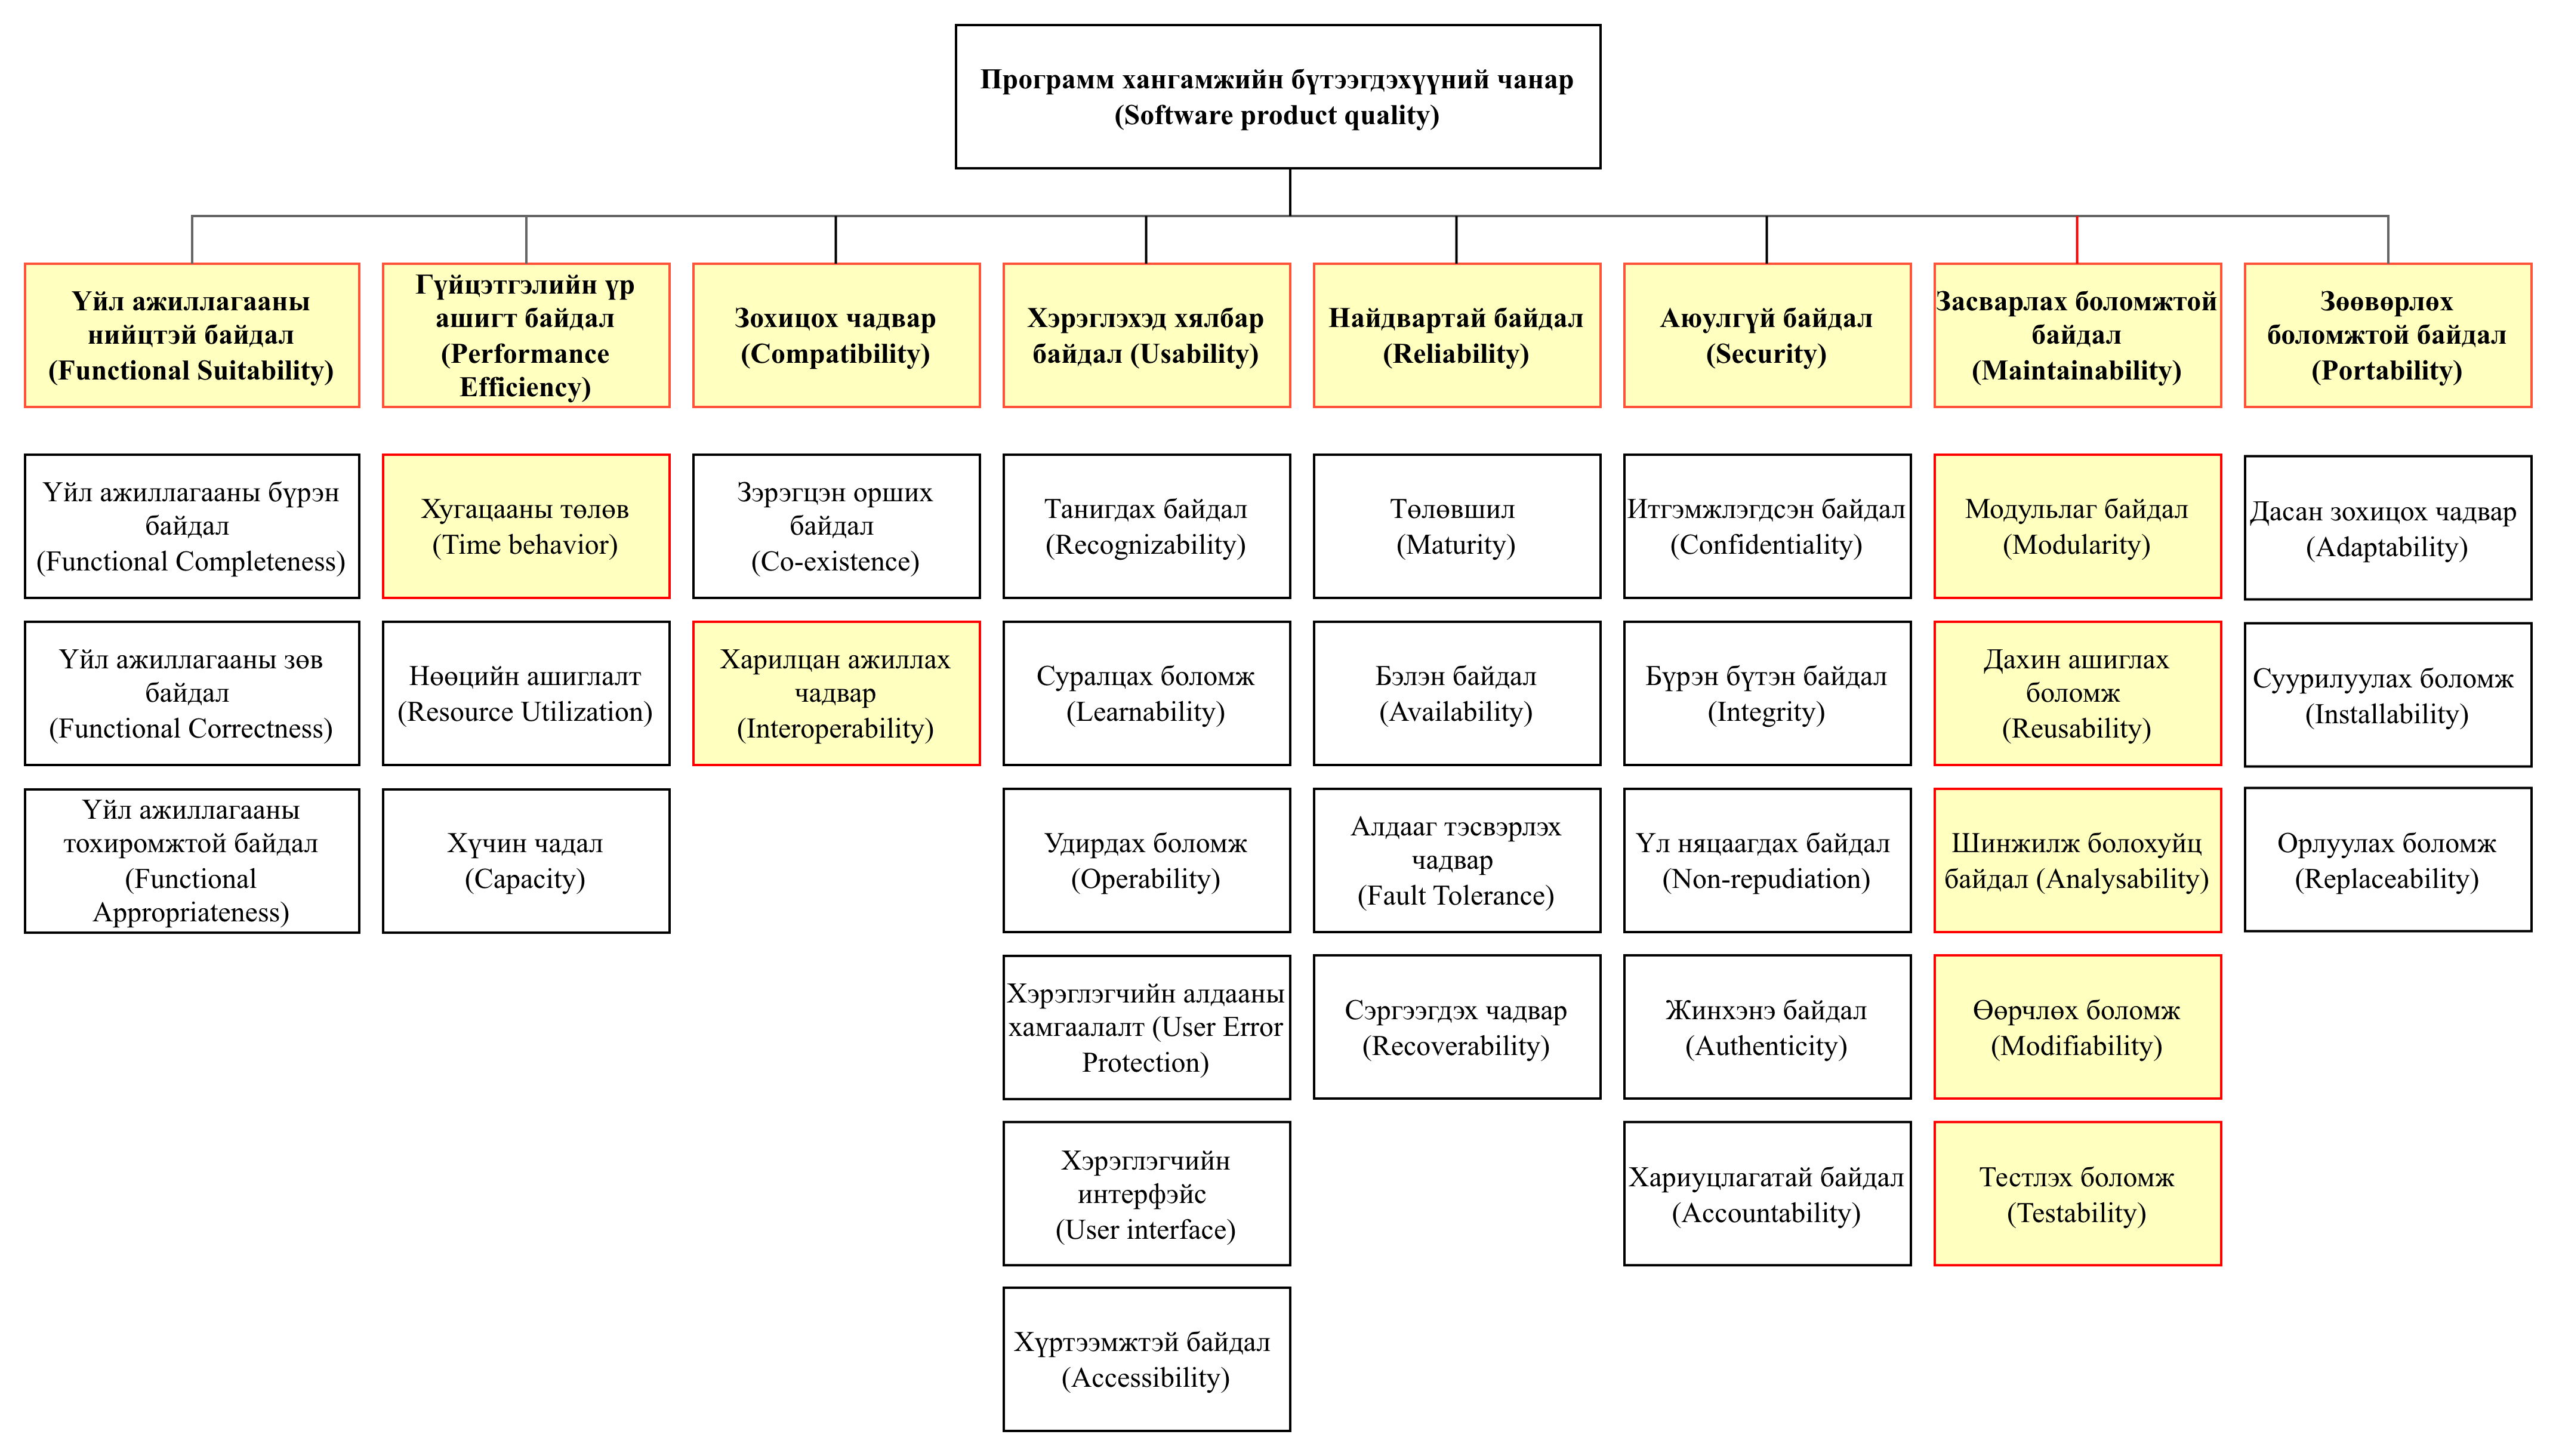
\includegraphics[width=17cm]{images/qa.png}
	\caption{Бүтээгдэхүүний чанарын загвар ба сонгосон чанарын үзүүлэлтүүд}
	\label{fig:qa}
\end{figure}
Энэхүү судалгаанд ашиглах сонгосон чанарын үзүүлэлтүүдийн талаар илүү сайн ойлголт өгөхийн тулд тэдгээрийн тодорхойлолт болон тайлбарыг дараах дэд хэсгүү- дэд орууллаа.
\subsection{Хугацааны төлөв (Time behavior)}
\cite{iso25010_2}-т энэ үзүүлэлтийг "тухайн бүтээгдэхүүн эсвэл систем нь өөрийн үйл ажиллагааг гүйцэтгэхдээ хариу үйлдэл үзүүлэх хугацаа, боловсруулалтын хурд болон нэвтрүүлэх чадвар нь тавигдсан шаардлагыг хэр зэрэг хангаж буй түвшин" гэж тодорхойлсон байдаг.

\subsection{Харилцан ажиллах чадвар (Interoperability)}
Энэ үзүүлэлт нь "хоёр буюу түүнээс дээш системүүд хоорондоо мэдээлэл солилцож, уг солилцсон мэдээллээ ашиглаж чадах түвшин"-г илэрхийлнэ \cite{iso25010_2}.

\subsection{Модульлаг байдал (Modularity)}
Энэ үзүүлэлтийг "систем эсвэл компьютерын программ нь аль нэг бүрэлдэхүүн хэсэгтээ өөрчлөлт оруулахад бусад хэсгүүддээ хамгийн бага нөлөө үзүүлэхүйц салангид хэсгүүдээс бүрдсэн байх хэмжүүр" гэж тодорхойлдог \cite{iso25010_2}. Энэ нь микрофронтенд архитектур руу амжилттай шилжихэд чухал үүрэг гүйцэтгэх гол үзүүлэлтүүдийн нэг юм.

\subsection{Дахин ашиглах боломж (Reusability)}
Энэ үзүүлэлтийг "аливаа нэг нөөц, бүрэлдэхүүнийг нэгээс олон системд, эсвэл өөр шинэ нөөц бүтээхэд ашиглаж болох түвшин" хэмээн тодорхойлдог \cite{iso25010_2}. Энэ нь микрофронтенд архитектурт шилжих процессад ихээхэн эерэг нөлөө үзүүлнэ гэж үздэг.

\subsection{Шинжилж болохуйц байдал (Analysability)}
Энэ үзүүлэлтийг "бүтээгдэхүүн эсвэл системийн аль нэг хэсэгт өөрчлөлт оруулахад гарах нөлөөллийг үнэлэх, доголдол болон алдааны шалтгааныг оношлох, эсвэл өөрчлөх шаардлагатай хэсгүүдийг тодорхойлох процесс хэр үр дүнтэй, үр ашигтай байх түвшин" гэж тодорхойлжээ \cite{iso25010_2}. Энэхүү үзүүлэлт нь кодод дүн шинжилгээ хийх болон алдааг олж засварлахад хэр хялбар байгаагаар илэрдэг.

\subsection{Өөрчлөх боломж (Modifiability)}
Энэ үзүүлэлтийг "бүтээгдэхүүн, системд шинээр алдаа доголдол үүсгэхгүйгээр, эсвэл одоо байгаа чанарыг нь бууруулахгүйгээр үр дүнтэй бөгөөд үр ашигтай өөрчлөлт оруулах боломжтой түвшин" хэмээн тодорхойлдог \cite{iso25010_2}. Хэрэглээний программын өөрчлөх боломж нь кодын санд өөрчлөлт оруулахад хэр хялбар байгааг харуулдаг үзүүлэлт юм.

\subsection{Тестлэх боломж (Testability)}
Энэ үзүүлэлтийг "систем, бүтээгдэхүүн эсвэл түүний бүрэлдэхүүн хэсгийн хувьд тестийн шалгуурыг тогтоож, уг шалгуурыг хангасан эсэхийг баталгаажуулах тестийг гүйцэтгэх боломжтой байдлын түвшин" гэж тодорхойлсон байдаг \cite{iso25010_2}. Өөрөөр хэлбэр, энэ нь тухайн бүрэлдэхүүн хэсэг, модулийг янз бүрийн тестийн аргуудаар хэр хялбар тестэлж болохыг илтгэнэ.

